% arara: pdflatex
% arara: pdflatex
% arara: makeindex: { sort: on, style: mychemistry_en.ist }
% arara: pdflatex
% --------------------------------------------------------------------------
% the MYCHEMISTRY package
%
%   create reaction schemes with LaTeX and chemfig
%
% --------------------------------------------------------------------------
% Clemens Niederberger
% Web:    https://www.bitbucket.org/cgnieder/mychemistry
% E-Mail: contact@mychemistry.eu
% --------------------------------------------------------------------------
% If you have any ideas, questions, suggestions or bugs to report, please
% feel free to contact me.
% --------------------------------------------------------------------------
% Copyright 2011--2012 Clemens Niederberger
%
% This work may be distributed and/or modified under the
% conditions of the LaTeX Project Public License, either version 1.3
% of this license or (at your option) any later version.
% The latest version of this license is in
%   http://www.latex-project.org/lppl.txt
% and version 1.3 or later is part of all distributions of LaTeX
% version 2005/12/01 or later.
%
% This work has the LPPL maintenance status `maintained'.
%
% The Current Maintainer of this work is Clemens Niederberger.
%
% This work consists of the files modiagram.sty, modiagram_en.tex,
% README and the derived file modiagram_en.pdf.
% --------------------------------------------------------------------------
% \errorcontextlines=999
\documentclass[toc=index,DIV10]{cnpkgdoc}
\docsetup{
  pkg = [draft]mychemistry,
  subtitle = Create Reaction Schemes with \LaTeXe\ and Chemfig ,
  code-box     = {
    skipbelow        = .5\baselineskip plus .5ex minus .5ex ,
    skipabove        = .5\baselineskip plus .5ex minus .5ex ,
    roundcorner      = 3pt ,
    innerleftmargin  = 1.5em ,
    innerrightmargin = 1.5em
  }
}

\usepackage{chemnum}
\usepackage{fnpct}
\usepackage{booktabs}
\usepackage{siunitx}

\chemsetup[chemformula]{format=\libertineLF}

\addcmds{
  @addtoreset,
  anywhere,
  arrow,
  branch,
  celsius,
  ch,
  chemabove,
  chemand,
  chembelow,
  chemfig,
  chemname,
  cmpd,
  colorlet,
  command,
  draw,
  elmove,
  floatstyle,
  fpch,
  fplus,
  fscrm,
  fscrp,
  Hpl,
  iupac,
  lewis,
  Lewis,
  listof,
  makeinvisible,
  makevisible,
  marrow,
  mch,
  mCsetup,
  mech,
  mesomeric,
  N,
  node,
  para,
  pch,
  phantom,
  reactant,
  restylefloat,
  setarrowlabel,
  setarrowlength,
  setarrowline,
  setatomsep,
  setatomsize,
  setbondlength,
  setbondshape,
  setcrambond,
  setmergelength,
  setrcndist,
  setrxnalign,
  setschemealign,
  setschemename,
  SI,
  text,
  therxnscheme,
  tikzset,
  trans,
  transition
}

\usepackage{makeidx}
\usepackage{filecontents}
\begin{filecontents*}{\jobname.ist}
 heading_prefix "{\\bfseries "
 heading_suffix "\\hfil}\\nopagebreak\n"
 headings_flag  1
 delim_0 "\\dotfill "
 delim_1 "\\dotfill "
 delim_2 "\\dotfill "
 delim_r "\\nohyperpage{\\textendash}"
 suffix_2p "\\nohyperpage{\\,f.}"
 suffix_3p "\\nohyperpage{\\,ff.}"
\end{filecontents*}

\makeindex

\begin{document}
\section{Licence and Requirements}\label{ssec:voraussetzungen}
Permission is granted to copy, distribute and/or modify this software under the
terms of the LaTeX Project Public License, version 1.3 or later
(\url{http://www.latex-project.org/lppl.txt}). This package has the status
``maintained.''

\mychemistry needs and loads the packages \paket{etoolbox}, \paket{float},
\paket{xkeyval}, \paket{chemmacros} and \paket{chemfig}. It also loads the 
TikZ-libraries \code{arrows}, \code{positioning}, \code{decorations.pathmorphing},
\code{shapes}, \code{calc}, \code{matrix}, \code{chains}, \code{scopes} and
\code{intersections}.

\mychemistry also loads \paket*{translations}\footnote{Part of the
\paket*{exsheets} package} for proper language support.

\section{Changes}
With v1.99 (=v2.0beta) package dependencies have changed so that \mychemistry
loads noticably less packages than before. Most important for you: it does \emph{not}
load \paket{mhchem} any more. This documentation uses \paket{chemmacros} instead
which is loaded by \mychemistry.

There are now considerably less package options as most of them are not needed
any more.

\mychemistry now provides proper language support, \eg, when used together with
\paket{babel}.

New is the command \cmd{setelmove}. The command \cmd{makevisible} now only has
an effect if the new option \key{draft} is used.

\section{Background}
\mychemistry provides two environments within which the mechanisms are created.
Both environments basically are \code{tikzpicture} environments. When this package
first was written \paket{chemfig} lacked the possibility of creating reaction
schemes itself. This was the motivation for me to get started on \mychemistry
which then rapidly grew and until now has its users.

The background has changed in August 2011, though. Then \paket{chemfig} v1.0 was
published and now provides simple but powerful macros to create reactions schemes.
They don't seem to to be used very often but I am advertising as much as I can.
Anyway, since then \mychemistry can be considered obsolete and is not actively
developed any more. The current release 1.99 (= 2.0beta) was due to an
incompatibilty with \paket{pdfpages} and a complete robustification of various
parts of the code.

\emph{Other than bug fixes this package will very likely \emph{not} be updated
any more}!

\section{Package options}\label{sec:paketoptionen}
\mychemistry has a few package options.
\begin{beschreibung}
  \option{strict} With this option all warning messages are turned into error
    messages.
  \option{draft} This option is an alias to \key{strict}. Additionally it enables
    the \cmd{makevisible} command.
  \option{final} This option is the opposite to \key{draft}, \ie, most error
    messages will be issued as warnings. It also disables the \cmd{makevisible}
    command.
  \option{placement}{<value>} Changes the default floating behaviour of \env{rxnscheme},
    see section~\ref{ssec:rxnscheme}.
\end{beschreibung}

\section{Usage}
\subsection{Basic Principle}
Within the \code{tikzpicture} reactants and arrows are placed as nodes on a
\code{chain}\footnote{Provided by the tikzlibrary `chains'}.

\begin{beispiel}
 \begin{tikzpicture}[start chain]
 \node [on chain] {A};
 \node [on chain] {B};
 \node [on chain] {C};
 \end{tikzpicture}
\end{beispiel}
This way there are several possibilities to place the nodes relative to the others.
\begin{beispiel}
 \begin{tikzpicture}[start chain=going right,node distance=5mm]
 \node [draw,on chain] {Hello};
 \node [draw,on chain] {World};
 \node [draw,continue chain=going below,on chain] {,};
 \node [draw,on chain] {this};
 \node [draw,on chain] {is};
 \end{tikzpicture}
\end{beispiel}

Above all \mychemistry uses the possibility of creating branches to the chain.
\begin{beispiel}
 \begin{tikzpicture}[start chain=going right,node distance=5mm]
  \node [draw,on chain] {A};
  \node [draw,on chain] {B};
 { [start branch]
  \node [on chain=going below] {1};
  \node [on chain=going below] {2};
 }
 { [start branch]
  \node [on chain=going above] {$\alpha$};
  \node [on chain=going above] {$\beta$};
 }
  \node [draw,on chain] {C};
 \end{tikzpicture}
\end{beispiel}
You don't have to understand that mechanism in detail but you should remember the
placement commands in the last example, because \mychemistry uses them in the same
way.

In some of the examples in this documentation the nodes are boxed with a coloured
frame (see section~\ref{ssec:makevisible}). This is done so one can see, which size
they have and which impact changes of the alignment have on them.

\subsection{How does it work?}
\subsubsection{Basic Commands}
There are two basic commands:
\begin{beschreibung}
  \Befehl{reactant}[<pos>,<name>,<tikz>]{<formula>}
  \Befehl{arrow}[<pos>,<type>,<length factor>,<name>,both,<tikz>]{<above>}\ma{<below>}
\end{beschreibung}

Schemes are created within the \env{rxn}{} environment. There you place reactants
and arrows.
\begin{beispiel}
 \begin{rxn}
  \reactant{ \chemfig{-[::30]-[::-60]OH} }
  \arrow{Ox.}{}
  \reactant{ \chemfig{-[::30]=_[::-60]O} }
 \end{rxn}
\end{beispiel}

When you don't use options reactants and arrows always are put to the right of
the last object. With the option \code{<pos>} you can change this behaviour.
\begin{beispiel}
  % positioning using key words
 \begin{rxn}
  \reactant{ \chemfig{-[::30]-[::-60]OH} }
  \arrow[below]{Ox.}{}
  \reactant[below]{ \chemfig{-[::30]=_[::-60]O} }
 \end{rxn}
 % positioning using an angle
 \begin{rxn}
  \reactant{ \chemfig{-[::30]-[::-60]OH} }
  \arrow[180]{}{Ox.}
  \reactant[180]{ \chemfig{-[::30]=_[::-60]O} }
 \end{rxn}
\end{beispiel}

\begin{table}
 \centering
 \begin{tabular}{>{\ttfamily}l*{2}{>{$}r<{$}}}
  \toprule
  {\normalfont key word} & \text{pos. angle} & \text{neg. angle} \\
  \midrule
  right       & 0   & \pm 360 \\
  right above & 45  & -315 \\
  above       & 90  & -270 \\
  above left  & 135 & -225 \\
  left        & 180 & -180 \\
  below left  & 225 & -135 \\
  below       & 270 & -90 \\
  below right & 315 & -45 \\
  \bottomrule
 \end{tabular}
 \caption{key words for positioning}\label{tab:keywords}
\end{table}

You can see in the last example that positioning can be realized through key
words (see table~\ref{tab:keywords}) like \code{below} or by using the angle
relative to the horizontal line. Every angle from the interval
$[\ang{-360};\ang{360}]$. \ang{0} corresponds to \code{right} which is the default
value. \emph{Positive angles} mean a turn \emph{counter clockwise}, negative ones
a turn clockwise -- like you're used to in mathematics.

\begin{beispiel}
 \begin{rxn}
  \reactant{ \chemfig{-[::30]-[::-60]OH} }
  \arrow[20]{Ox.}{}
  \reactant[20]{ \chemfig{-[::30]=_[::-60]O} }
 \end{rxn}
 \begin{rxn}
  \reactant{ \chemfig{-[::30]-[::-60]OH} }
  \arrow[-20]{Ox.}{}
  \reactant[-20]{ \chemfig{-[::30]=_[::-60]O} }
 \end{rxn} 
\end{beispiel}

\subsubsection{Positioning}
Reactants and arrows cannot only be positioned through key words and angles. They
can refer to another reactant or arrow.
\begin{beispiel}
 \begin{rxn}
  \reactant[,start]{ \chemfig{R-[::30](-[::60]R|^1) (-[::-120]R|^2)-[::-60]OH} }
  \arrow[40]{\tiny$\text{R}^1=\text{H}$} {\tiny$\text{R}^2=\text{H}$}
  \reactant[40]{ \chemfig{R-[::30]=_[::-60]O} }
  \arrow[start.0]{\tiny$\text{R}^1=\text{alkyl}$} {\tiny$\text{R}^2=\text{H}$}
  \reactant{ \chemfig{R-[::30](-[::60]R)=_[::-60]O} }
  \arrow[start.-40,-|>]{\tiny$\text{R}^1=\text{alkyl}$} {\tiny$\text{R}^2=\text{Alkyl}$}
 \end{rxn}
\end{beispiel}
In the last example the first reactant got the \code{<name>} \code{start}. The
arrows in lines 5 and 7 now could refer to it. A \emph{previously given name} can
act as an anchor for later reactants or arrows, if the positioning is written like
\code{<anchor>.<angle>}.

Arrows can be given names, too. The anchor point of an arrow always is in the
middle of the arrow line and has \emph{no} size.
\begin{beispiel}
 \begin{rxn}
  \reactant{\chemfig{[:60]-(-[::60])=[::-60](-[::-60])-}}
  \arrow[,,,arrow]{}{}
  \reactant[arrow.90]{\ch{H2O}}
 \end{rxn}
\end{beispiel}

Using this kind of positioning does \emph{not} break the chain.
\begin{beispiel}[code only]
 \begin{rxn}
  \reactant[,a]{A}
  \arrow{}{}
  \reactant{B}
  \arrow[a.-90]{}{}
  \reactant[-90]{C}
  \arrow[a.180]{}{}
  \reactant[180]{D}
 \end{rxn}
\end{beispiel}

All seven objects of this example are logically speaking part of the same chain.
The next object is placed to the right of the last one if no positioning is used.
\begin{rxn}
 \tikzset{nummer/.style={circle,fill=gray!30,draw=gray,minimum size=3.5mm}}
 \reactant[,a]{A}\arrow[,,,pa]{}{}\reactant[,b]{B}
 \arrow[a.-90,,,pb]{}{}\reactant[-90,c]{C}
 \arrow[a.180,,,pc]{}{}\reactant[180,d]{D}
 \anywhere{a.45,,nummer}{1}
 \anywhere{pa.90,,nummer}{2}
 \anywhere{b.45,,nummer}{3}
 \anywhere{pb.0,,nummer}{4}
 \anywhere{c.45,,nummer}{5}
 \anywhere{pc.90,,nummer}{6}
 \anywhere{d.45,,nummer}{7}
\end{rxn}

\subsubsection{Branches}
To break a chain you use the command
\begin{beschreibung}
 \Befehl{branch}[<pos>,<name>,<tikz>]{<formulae>}
\end{beschreibung}
The positioning of a branch is slightly different from earlier objects, although
the syntax is similar. A branch has two additional ways of positioning. Every
positioning that refers to an anchor cause that the branch is not a part of the
chain but is a real branch.
\begin{description}
 \item[\code{<angle>}] on the chain
 \item[\code{<key>}] on the chain
 \item[\code{<anchor>.<angle>}] not on the chain
 \item[\code{on chain=going <key>}]on the chain
 \item[\code{<key>=of <anchor>}] not on the chain
\end{description}
As \code{<key>} you again use the values from table~\ref{tab:keywords}.

\begin{beispiel}
 \begin{rxn}
  \reactant{ \chemfig{-[::30]-[::-60]OH} }
  \arrow{}{}
  \reactant[,carbonyl]{ \chemfig{-[::30]=_[::-60]O} }
  \branch[carbonyl.-90]{
    \arrow[-90,<=>]{\ch{NH2R}}{}
    \reactant[-90]{ \chemfig{-[::30]=_[::-60]N(-[6]H)-[::60]R} }
  }
  \arrow{}{}
  \reactant{ \chemfig{-[::30](-[::60]OH)=_[::-60]O} }
 \end{rxn}
\end{beispiel}

Please note that in the last example the arrow and the reactant placed after
branch continue the original chain.
\begin{beispiel}[code only]
 \begin{rxn}
  \reactant[,a]{A}
  \arrow{}{}
  \reactant{B}
  \branch[a.-90]{
    \arrow[-90]{}{}
    \reactant[-90]{C}
  }
  \arrow[a.180]{}{}
  \reactant[180]{D}
 \end{rxn}
\end{beispiel}

The chain is broken by the branch which starts a new chain itself.
\begin{rxn}
 \tikzset{nummer/.style={circle,fill=gray!30,draw=gray,minimum size=3.5mm,overlay}}
 \reactant[,a]{A}\arrow[,,,pa]{}{}\reactant[,b]{B}
 \branch[a.-90]{
   \arrow[-90,,,pb]{}{}\reactant[-90,c]{C}
    \anywhere{pb.0,,nummer}{a}
    \anywhere{c.45,,nummer}{b}
 }
 \arrow[a.180,,,pc]{}{}\reactant[180,d]{D}
 \anywhere{a.45,,nummer}{1}
 \anywhere{pa.90,,nummer}{2}
 \anywhere{b.45,,nummer}{3}
 \anywhere{pc.90,,nummer}{4}
 \anywhere{d.45,,nummer}{5}
\end{rxn}

Using \cmd{branch} allows to create schemes with several branches:
\begin{beispiel}
 \begin{rxn}
  \reactant{ \chemfig{-[::30]-[::-60]OH} }
  \arrow{}{}
  \reactant[,carbonyl]{ \chemfig{-[::30]=_[::-60]O} }
  \arrow[-90]{}{}
  \reactant[-90]{ \chemfig{-[::30](-[::60]OH)=_[::-60]O} }
  \branch[right=of carbonyl]{
    \arrow[,<=>,1.12]{\ch{NH2R}}{}
    \reactant{ \chemfig{-[::30]=_[::-60]N(-[6]H)-[::60]R} }
  }
  \branch[below right=of carbonyl]{
    \arrow[-45,<=>,1.12]{ \chemfig{[,.75]-[::30]-[::-60]OH} }{}
    \reactant[-45]{ \chemfig{-[::30](-[::60]O-[::-60]-[::-60])-[::-60]OH} }
  }
  \arrow[carbonyl.90]{ \chemfig{[,.75]-[::30]=_[::-60]O}/\Hpl }{}
  \reactant[90]{ \chemfig{-[::30](-[::60]OH)-[::-60]-[::60]=[::60]O} }
  \arrow{$-\ch{H2O}$}{}
  \reactant{ \chemfig{-[::30]=[::-60]-[::60]=[::60]O} }
 \end{rxn}
\end{beispiel}

\subsubsection{Numbered Schemes}
There is another environment to create schemes.
\begin{beschreibung}
 \Umg{rxnscheme}[<label>,<placement>,<alignment>,<skale factor>,<title>]{<caption>}
\end{beschreibung}

This is a floating environment for scheme, which can be given a \code{<caption>},
a \code{<label>} and the common placement identifiers like \code{htp} (default).
\begin{beispiel}[code and float]
\begin{rxnscheme}{Keto-Enol-tautomerism}
 \reactant{ \chemfig{=[::30]-[::-60]OH} }
 \arrow[,<=>]{}{}
 \reactant{ \chemfig{-[::30]=[::-60]O} }
\end{rxnscheme}
\end{beispiel}

\subsection{Predefined Values}
There are some predefined values that are basically due to my personal taste. But
of course you can change them according to your requirements. For \paket{chemfig}%
-formul\ae\ \emph{inside of \mychemistry environments} some values are predefined
as follows:
\begin{beispiel}[code only]
 \setatomsep{1.8em}
 \setcrambond{3pt}{0.5pt}{1pt}
\end{beispiel}
Outside the \mychemistry environments the defaults of \paket{chemfig} still are
set.
\begin{beispiel}
 \begin{rxn}
  \reactant{\chemfig{**6(------)}}
 \end{rxn}
 \chemfig{**6(------)}
\end{beispiel}

\mychemistry's defaults can be changed with these commands:
\begin{beschreibung}
 \Befehl{setbondlength}{<length>}
 \Befehl{setbondshape}{<base length>}\ma{<dash thickness>}\ma{<dash spacing>}
 \Befehl{setatomsize}{<font size>}
\end{beschreibung}
With these commands the parameters are changed \emph{for all following}
\mychemistry environments. If you leave the arguments empty default values are
restored. Default for \cmd{setatomsize} is \cmd{small}.

\begin{beispiel}
 \setbondlength{2.1em}\setbondshape{5pt}{1pt}{2pt}\setatomsize{\Large}
 \begin{rxn}
  \reactant{\chemfig{-[::30](<[::60])-[::-60](<:[::-60])-[::60]A}}
 \end{rxn}
 \setbondlength{}\setbondshape{}{}{}\setatomsize{}
 \begin{rxn}
  \reactant{\chemfig{-[::30](<[::60])-[::-60](<:[::-60])-[::60]A}}
 \end{rxn}
\end{beispiel}

If you only want to change the parameters of a single environment you can use
\paket{chemfig}'s commands and \LaTeX's fontsize commands \emph{inside the
environment}.
\begin{beispiel}
 \begin{rxn}
  \setatomsep{2.1em}\setcrambond{5pt}{1pt}{2pt}\Large
  \reactant{\chemfig{-[::30](<[::60])-[::-60](<:[::-60])-[::60]A}}
 \end{rxn}
 \begin{rxn}
  \reactant{\chemfig{-[::30](<[::60])-[::-60](<:[::-60])-[::60]A}}
 \end{rxn}
\end{beispiel}

The default length of reaction arrows is \SI{4}{em}, the default line width is
\code{semithick} and the default label distance is \SI{0.2}{em}. You can change
these default values with the commands
\begin{beschreibung}
 \Befehl{setarrowlength}{<length>}
 \Befehl{setarrowline}{<line width>}
 \Befehl{setarrowlabel}{<label distance>}
\end{beschreibung}
or with
\begin{beschreibung}
 \befehl{mCsetup}{<options>} valid options are:
 \Option{arrowlength}{<length>}
 \Option{arrowline}{<line width>}
 \Option{arrowlabel}{<label distance>}
\end{beschreibung}

\section{Advanced Usage, Usage with \TikZ}
The biggest problem with \mychemistry usually is the correct positioning of
reactants and arrows. Section~\ref{ssec:ausrichtungsfrage} looks a little bit
into this topic.

Some of the commands can be given \TikZ code as third optional argument. More
precisely you can use the same \TikZ keys there as you would with a \cmd{node}
inside a \code{tikzpicture}. If a node is placed with \cmd{node}\oa{<tikz>}%
\da{<placement>}\ma{<anything>} then \code{<tikz>} is about the same in \eg
\cmd{reactant}[,,<tikz>]{}. With this you can customize your scheme in many ways.

\subsection{The Alignment Question}\label{ssec:ausrichtungsfrage}
Since reactants, arrows and branches are aligned centered to the referred object
the default alignment not always produces nice results.
\begin{beispiel}
 \makevisible
 \begin{rxn}
  \reactant{ \chemname{\chemfig{*6(-=-=-=)}}{benzene \cmpd{benzene}} }
  \arrow{}{}
  \reactant{ \chemname{\chemfig{*6(-=-=(-Br)-=)}}{bromobenzene \cmpd{bromobenzene}} }
 \end{rxn}
\end{beispiel}
As you can see both reactants are not aligned equally to the arrow as far as the
benzene ring is concerned. The first reactant seems to be shifted up. Trying to
solve this with \TikZ code fails:

\begin{beispiel}
 \makevisible
 \begin{rxn}
  \reactant[,,yshift=-1em]{ \chemname{\chemfig{*6(-=-=-=)}}{benzene \cmpd{benzene}} }
  \arrow{}{}
  \reactant{ \chemname{\chemfig{*6(-=-=(-Br)-=)}}{bromobenzene \cmpd{bromobenzene}} }
 \end{rxn}
\end{beispiel}
This is, because the first reactant is shifted with the respect to the object it
refers to. Since it is the first object on the chain itself it isn't shifted a
all. The following arrow always is centered to the object before.
\begin{beispiel}
 \makevisible
 \begin{rxn}
  \reactant{A}
  \chemand
  \reactant[,,yshift=1em]{B}
  \arrow{}{}
 \end{rxn}
\end{beispiel}
Since there is no possibility to change the alignment of the arrow itself what
you can do is put it inside a branch.
\begin{beispiel}
 \makevisible
 \begin{rxn}
  \reactant{A}
  \chemand
  \reactant[,,yshift=1em]{B}
  \branch[,,yshift=-1em]{\arrow{}{}}
 \end{rxn}
 \begin{rxn}
  \reactant{ \chemname{\chemfig{*6(-=-=-=)}}{benzene \cmpd{benzene}} }
  \branch[,,yshift=1em]{\arrow{}{}}
  \reactant{ \chemname{\chemfig{*6(-=-=(-Br)-=)}}{bromobenzene \cmpd{bromobenzene}} }
 \end{rxn}
\end{beispiel}
For the last example this isn't the best solution though because exact alignment
needs lots of tries until you get the required result. There is another solution:
an invisible bromine to the first benzene.
\begin{beispiel}
 \makevisible
 \begin{rxn}
  \reactant{ \chemname{\chemfig{*6(-=-=(-[,,,,draw=none]\phantom{Br})-=)}}{benzene \cmpd{benzene}} }
  \arrow{}{}
  \reactant{ \chemname{\chemfig{*6(-=-=(-Br)-=)}}{bromobenzene \cmpd{bromobenzene}} }
 \end{rxn}
\end{beispiel}
In other cases, too, an invisible substituent should be preferred over \TikZ code
since it's easier and more precise:
\begin{beispiel}
 \makevisible
 default:
 \begin{rxn}
  \reactant{\chemfig{-[:-30]-[:30](=[2]O)-[:-30]OH}}
  \chemand
  \reactant{\chemfig{HO-[:30]-[:-30]-[:30]}}
  \arrow{[\Hpl]}{\SI{200}{\celsius}}
  \reactant{\chemfig{-[:-30]-[:30](=[2]O)-[:-30]O-[:30]-[:-30]-[:30]}}
 \end{rxn}
 hydroxy groups at the same height through TikZ:
 \begin{rxn}
  \reactant{\chemfig{-[:-30]-[:30](=[2]O)-[:-30]OH}}
  \chemand[,,yshift=-1.2em]
  \reactant[,,yshift=.12em]{\chemfig{HO-[:30]-[:-30]-[:30]}}
  \branch[,,yshift=1.08em]{\arrow{[\Hpl]}{\SI{200}{\celsius}}}
  \reactant{\chemfig{-[:-30]-[:30](=[2]O)-[:-30]O-[:30]-[:-30]-[:30]}}
 \end{rxn}
 hydroxy groups at the same height through an invisible substituent:
 \begin{rxn}
  \reactant{\chemfig{-[:-30]-[:30](=[2]O)-[:-30]OH}}
  \chemand
  \reactant{\chemfig{HO-[:30](=[2,,,,draw=none]\phantom{O})-[:-30]-[:30]}}
  \arrow{[\Hpl]}{\SI{200}{\celsius}}
  \reactant{\chemfig{-[:-30]-[:30](=[2]O)-[:-30]O-[:30]-[:-30]-[:30]}}
 \end{rxn}
\end{beispiel}

I'm afraid that in many other cases you'll have to play with \code{xshift} and
\code{yshift}, though, until the scheme looks the way you want.

\subsection{Using \TikZ to Achieve Other Results}
You could, just for fun?, change the looks of a molecule with \TikZ.
\begin{beispiel}
 \begin{rxn}
  \reactant[,,->,green!45!blue!55]{ \chemfig{*6(---(-)---)} }
 \end{rxn}
 \chemfig[->,green!45!blue!55]{*6(---(-)---)}
\end{beispiel}
The last example is not very good, of course, since you can achieve the same result
using \paket{chemfig}'s own possibilities. But other cases are imaginable: for
example one could define a style with which reactants are shown:
\begin{beispiel}
 \colorlet{mCgreen}{green!50!gray}
 \colorlet{mCblue}{cyan!50!gray}
 \colorlet{mCred}{magenta!50!gray}
 \colorlet{mCyellow}{yellow!50!gray}
 \begin{rxn}
  \tikzset{reactant/.style={draw=#1,fill=#1!10,inner sep=1em,minimum height=10em,minimum width=12em,rounded corners}}
  \reactant[,cytosine,reactant=mCred]{\chemfig{H-[:30]N*6(-(=O)-N=(-NH_2)-=-)}}
  \anywhere{cytosine.-90,,yshift=-2mm}{Cytosine}
  \reactant[,thymine,reactant=mCyellow]{\chemfig{H-[:30]N*6(-(=O)-N(-H)-(=O)-(-CH_3)=-)}}
  \anywhere{thymine.-90,,yshift=-2mm}{Thymine}
  \reactant[cytosine.-90,adenine,yshift=-2em,reactant=mCblue]{\chemfig{[:-36]*5(-N(-H)-*6(-N=-N=(-NH_2)--)--N=)}}
  \anywhere{adenine.-90,Guanin,yshift=-2mm}{Adenine}
  \reactant[,guanine,reactant=mCgreen]{\chemfig{[:-36]*5(-N(-H)-*6(-N=(-NH_2)-N(-H)-(=O)--)--N=)}}
  \anywhere{guanine.-90,,yshift=-2mm}{Guanine}
 \end{rxn}
\end{beispiel}
This way certain parts of a scheme could be emphasized:
\begin{beispiel}
 \begin{rxn}
  \setatomsep{1.5em}
  \colorlet{mCgreen}{green!50!gray}
  \tikzset{emph/.style={draw=mCgreen,fill=mCgreen!10,inner sep=1em}}
  \reactant[,lineOne]{\chemfig{R^1-[:30](=[@{b1}2]O)-[:-30]O-H}}
  \arrow[,<=>]{\chemfig{@{Hpl1}\Hpl}}{}
  \branch[,,emph]{
    \reactant{\chemfig{R^1-[:30]@{C1}(-[2]O-[:30]H)(-[6,.5,,,draw=none]\fplus)-[:-30]O-H}}
    \arrow[,<=>,2]{\chemfig{[:30]H-@{O1}O-[::-60]-R^2}}{}
    \reactant{\chemfig{R^1-[:30](-[2]O-[:30]H)(-[6]@{O2}O-[:-150]H)-[:-30]@{O3}\chemabove{O}{\fplus}(-[@{b2}6]H)-[:30]-[:-30]R^2}}
  }
  \anywhere{lineOne.-90,lineTwo,xshift=-3em,yshift=-7em}{}
  \arrow[lineTwo.0,<=>]{$-$\Hpl/\chemfig{@{Hpl2}\Hpl}}{}
  \reactant{\chemfig{R^1-[:30](-[@{b3}2]O-[@{b4}:30]H)(-[@{b5}6]@{O4}\chembelow{O}{\fplus}(-[:-30]H)-[:-150]H)-[:-30]O-[:30]-[:-30]R^2}}
  \arrow[,<=>,2]{$- \ch{H+} - \ch{H2O}$}{}
  \reactant{\chemfig{R^1-[:30](=[2]O)-[:-30]O-[:30]-[:-30]R^2}}
  \anywhere{lineTwo.-90}{
    \elmove{b1}{10:5mm}{Hpl1}{135:1cm}
    \elmove{O1}{135:1.5cm}{C1}{30:5mm}
    \elmove{O2}{-90:3cm}{Hpl2}{90:2cm}
    \elmove{b2}{0:5mm}{O3}{-10:5mm}
    \elmove{b4}{-40:5mm}{b3}{0:5mm}
    \elmove{b5}{-30:5mm}{O4}{-10:5mm}
  }
 \end{rxn}
\end{beispiel}

\section{Alphabetical Command Reference}
In the following section every command is explained.

\subsection{anywhere}\label{ssec:anywhere}
Sometimes it might be useful to be able to place a reactant or anything else off
the chain.
\begin{beschreibung}
 \Befehl{anywhere}{<pos>,<name>,<tikz>}\ma{<something>}
\end{beschreibung}
For this case there's \cmd{anywhere}. It is positioned with \code{<pos>} similar
to \cmd{branch}.
\begin{description}
 \item[\code{<anchor>.<angle>}] not on the chain
 \item[\code{on chain=going <key>}] on the chain
 \item[\code{<key>=of <anchor>}] not on the chain
\end{description}
Please be aware that \code{<pos>} cannot be left empty.

\begin{beispiel}
 \begin{rxn}
  \reactant[,carbonyl_A]{\chemfig{R_2C=O}}
  \anywhere{above=of carbonyl_A}{\chemfig{H-[:-30]O-[:30]H}};
 \end{rxn}
\end{beispiel}
You can use this command \eg for placing labels next to reactants.
\begin{beispiel}
 \begin{rxn}
  \reactant[,ketone]{\chemfig{H-\chemabove{C}{\hspace*{5mm}\scriptstyle\alpha}(-[2]H)(-[6,,,2]{}|{\textcolor{blue}H})-C(=[:60]\lewis{02,O})-[:-60]C|H_3}}
  \anywhere{below=of ketone}{$+ \ch[format=\color{blue}]{OH-}$}
  \arrow[,<=>]{\tiny slow}{}
  \mesomeric[,mesomer]{
    \reactant[,carbanion]{\chemfig{H_2|\chemabove[3pt]{\lewis{2,C}}{\fscrm}-C(=[:60]\lewis{02,O})-[:-60]C|H_3}}
    \marrow
    \reactant[,enolate]{\chemfig{H_2C=C(-[:60]\chemabove{\lewis{024,O}}{\hspace*{5mm}\fscrm})-[:-60]C|H_3}}
  }
  \anywhere{above=of enolate}{\tiny enolate ion}
  \anywhere{above=of carbanion}{\tiny carbanion}
  \anywhere{below=of mesomer}{$+ \ch[format=\color{blue}]{H2O}$}
 \end{rxn}
\end{beispiel}
You can find many further examples for the usage of \cmd{anywhere} in \code{examples.tex}
or \code{examples.pdf}, respectively.

\subsection{\cmd{arrow}}\label{ssec:arrow}
Reaction arrows are created with \cmd{arrow}.
\begin{beschreibung}
 \Befehl{arrow}[<pos>,<type>,<length factor>,<name>,both,<tikz>]{<above>}\ma{<below>}
\end{beschreibung}

\subsubsection{Options}
There are a number of options to customize the arrows. The options must be used
in the right order, separated with commas.
\begin{enumerate}
\item\code{<pos>} -- possible values:
 \begin{rxn}
  \setarrowlength{2.5em}
  \dummy[a]
  \arrow{}{}\reactant{right = \ang{0}}
  \branch[above right=of a]{\arrow[above right]{}{}\reactant[above right,,overlay]{above right = \ang{45}}}
  \branch[above=of a]{\arrow[above]{}{}\reactant[above,,overlay]{above = \ang{90}}}
  \branch[above left=of a]{\arrow[above left]{}{}\reactant[above left,,overlay]{above left = \ang{135}}}
  \branch[left=of a]{\arrow[left]{}{}\reactant[left,,overlay]{left = \ang{180} = \ang{-180}}}
  \branch[below left=of a]{\arrow[below left]{}{}\reactant[below left,,overlay,xshift=-2em]{below left = \ang{225} = \ang{-135}}}
  \branch[below=of a]{\arrow[below]{}{}\reactant[below,,overlay]{below = \ang{270} = \ang{-90}}}
  \branch[below right=of a]{\arrow[below right]{}{}\reactant[below right,,overlay,xshift=2em]{below right = \ang{315} = \ang{-45}}}
 \end{rxn}
 Additionally you can use every angle from the interval $[\ang{-360};\ang{360}]$.
 
 You can also use an angle with respect to an object that's been named with
 \code{<name>}: \code{<name>.<angle>}. This means the arrow is placed in an
 angle of \code{<angle>} next to \code{<name>}. You can find lots of examples in
 \code{examples.tex} or\code{examples.pdf}, respectively.
\item\code{<type>} -- possible values:
 \begin{rxn}
  \dummy[a]
  \branch[below=of a,b,yshift=.5em]{\arrow{}{}\reactant{\ttfamily -\textgreater}}
  \branch[below=of b,c,yshift=.5em]{\arrow[,<-]{}{}\reactant{\ttfamily \textless-}}
  \branch[below=of c,d,xshift=.25em,yshift=.5em]{\arrow[,<->]{}{}\reactant{\ttfamily \textless-\textgreater}}
  \branch[below=of d,e,yshift=.5em]{\arrow[,<=>]{}{}\reactant{\ttfamily \textless=\textgreater}}
  \branch[below=of e,f,xshift=.25em,yshift=.5em]{\arrow[,<=>>]{}{}\reactant{\ttfamily \textless=\textgreater{}\textgreater}}
  \branch[below=of f,g,yshift=.5em]{\arrow[,<<=>]{}{}\reactant{\ttfamily \textless{}\textless=\textgreater}}
  \branch[below=of g,h,xshift=-.25em,yshift=.5em]{\arrow[,-|>]{}{}\reactant{\ttfamily -\textbar\textgreater}}
  \branch[below=of h,,yshift=.5em]{\arrow[,-+>]{ }{ }\reactant{\ttfamily -+\textgreater}}
 \end{rxn}
\item\code{<length factor>} -- this factor multiplies with the arrow length
  (\SI{4}{em} with factor = $1.0$, default)
\item\code{<name>} -- can be used to give the arrow an anchor, to which another
  object can refer.
\item\code{both}-- this gives both nodes within which the labels are written the
  same size.
\item\code{<tikz>} -- you can modify the arrow with \TikZ keys. Not all \TikZ
  keys have an effect, though. You can't shift arrows with \code{shift=<coord>},
  for example.
\end{enumerate}
\begin{beispiel}
  \begin{rxn}
  \arrow[,,.25]{M}{}\arrow[,,.5]{MM}{}\arrow[,,.75]{MMM}{}\arrow{MMMM}{}\arrow[,,1.125]{MMMMM}{}\arrow[,,1.25]{MMMMM}{}
 \end{rxn}
\end{beispiel}
Please note, that the labels \code{<above>} and \code{<below>} are rotated with
the arrow. At an angle of \ang{180} \code{<above>} actually is \emph{below} the arrow.
\begin{beispiel}
 \begin{rxn}
  \setarrowlength{2.5em}
  \dummy[a]
  \arrow{a}{b}
  \arrow[a.45]{a}{b}
  \arrow[a.90]{a}{b}
  \arrow[a.135]{a}{b}
  \arrow[a.180]{a}{b}
  \arrow[a.225]{a}{b}
  \arrow[a.270]{a}{b}
  \arrow[a.315]{a}{b}
 \end{rxn}
\end{beispiel}

You need to be aware of one or two points, when using the arrow type \code{-+>}:
if you leave the labels empty, the arrow is the same as \code{->}. The first label
is the one added to the reaction, the second the one subtracted. If you use only
one of the labels only the corresponding arrow part is drawn.
\begin{beispiel}
 corresponds \verb"->":
 \begin{rxn}
  \arrow[,-+>]{}{}
 \end{rxn}
 add:
 \begin{rxn}
  \arrow[,-+>]{a}{}
 \end{rxn}
 subtract:
 \begin{rxn}
  \arrow[,-+>]{}{b}
 \end{rxn}
 both add and subtract:
 \begin{rxn}
  \arrow[,-+>]{a}{b}
 \end{rxn}
 Blanks are \emph{not} an empty label:
 \begin{rxn}
  \arrow[,-+>]{ }{ }
 \end{rxn}
\end{beispiel}

You can change the appearance of an arrow with \TikZ keys:
\begin{beispiel}
 \begin{rxn}
  \mCsetup{arrowlabel=.7em,arrowlength=6em}
  \reactant{A}
  \arrow[20,,,,,decorate,decoration=snake,blue]{a}{b}
  \reactant[20]{A$^*$}
 \end{rxn}
\end{beispiel}

\subsubsection{Alignment}
If an arrow is placed inside a branch the alignment of the branch may be
determined by the size of the label nodes. If the two labels have a different
size, alignment can go wrong.
\begin{beispiel}
 \makevisible
 \begin{rxn}
  \reactant[,a]{A}
  \arrow{}{}
  \branch[below=of a]{
    \arrow[-90]{\chemfig{-[::30]-[::-60]OH}}{}
  }
 \end{rxn}
 \makeinvisible
\end{beispiel}
By using the option \code{both} both nodes get the same size. This can correct
the alignment.
\begin{beispiel}
 \makevisible
 \begin{rxn}
  \reactant[,a]{A}
  \arrow{}{}
  \branch[below=of a]{
   \arrow[-90,,,,both]{\chemfig{-[::30]-[::-60]OH}}{}
  }
 \end{rxn}
 \makeinvisible
\end{beispiel}
There's more to the question of alignment in section~\ref{sssec:branch_ausrichtung}.

\subsubsection{Appearance}
You can change the general appearance of arrows with \cmd{setarrowlength}
(section~\ref{ssec:setarrowlength}) and \cmd{setarrowline} (section~\ref{ssec:setarrowline}).

\subsection{\cmd{branch}}\label{ssec:branch}
\cmd{branch} is used to, well, create a branch to a reaction.
\begin{beschreibung}
 \Befehl{branch}[<pos>,<anchor>,<tikz>]{<branch code>}
\end{beschreibung}
For \cmd{branch} positioning an anchor is important. Let's take a look at an example:
\begin{beispiel}
 \begin{rxn}
  \reactant[,start]{\chemfig{-[::30]=_[::-60](-[::-60])-[::60]}}
  \arrow[,,.75]{\ch{HCl}}{}
  \reactant{\chemfig{-[::30]-[::-60](-[::120]Cl)(-[::-60])-[::60]}}
  \chemand
  \reactant{\chemfig{-[::30](-[::60]Cl)-[::-60](-[::-60])-[::60]}}
  \branch[below right=of start]{
    \arrow[-45,,.75]{\ch{H2O}}{}
    \reactant[-45]{\chemfig{-[::30]-[::-60](-[::120]OH)(-[::-60])-[::60]}}
    \chemand
    \reactant{\chemfig{-[::30](-[::60]OH)-[::-60](-[::-60])-[::60]}}
  }
 \end{rxn}
\end{beispiel}
The first reactant got the anchor \code{start} (line 2, also see
section~\ref{ssec:reactant}). \cmd{branch} now refers to it in its alignment
(line 7). If you don't use the alignment reference to an anchor you automatically
refer to the last \cmd{reactant} or \cmd{arrow}. If you don't use alignment at all,
then the branch is aligned to the right of the last \cmd{reactant} or \cmd{arrow}.
\begin{beispiel}
 \begin{rxn}
  \reactant{ \chemfig{CH_2=CH-OH} }
  \arrow[,<=>,.5]{}{}
  \branch{ \reactant{ \chemfig{CH_3-CH=O} } }
 \end{rxn}
\end{beispiel}

\subsubsection{Positioning}\label{sssec:branch_positionierung}
There are several ways to position a branch. It can either be part of the chain
or be a real branch.
\begin{description}
 \item[\code{<angle>}] on the chain
 \item[\code{<key>}] on the chain
 \item[\code{<anchor>.<angle>}] not on the chain
 \item[\code{on chain=going <key>}] on the chain
 \item[\code{<key>=of <anchor>}] not on the chain
\end{description}

The default behaviour is equal to \cmd{branch}[0]{}. In different situations
different ways can be favoured. For example if you want to use \cmd{branch} to
shift an arrow it can still be part of the chain.
\begin{beispiel}
 \begin{rxn}
  \reactant{A}
  \branch[,,yshift=1em]{\arrow{}{}}
  \reactant[,,yshift=-1em]{B}
 \end{rxn}
\end{beispiel}

If you like to start a real branch it \emph{does} matter which way you use.
\begin{beispiel}
 \makevisible
 \begin{rxn}
  \reactant[,a]{\chemfig{[:30]--[::-60]-OH}}
  \arrow{}{}
  \branch[a.-45]{\arrow[-45]{}{}}
 \end{rxn}
 \begin{rxn}
  \reactant[,a]{\chemfig{[:30]--[::-60]-OH}}
  \arrow{}{}
  \branch[below right=of a]{\arrow[-45]{}{}}
 \end{rxn}
\end{beispiel}

If a reactant isn't squared or circled \ang{-45} does not mean the same as
``below right.''
\begin{beispiel}
 \makevisible
 \begin{rxn}
  \reactant[,a,circle]{\chemfig{[:30]--[::-60]-OH}}
  \arrow{}{}
  \branch[a.-45]{\arrow[-45]{}{}}
 \end{rxn}
 \begin{rxn}
  \reactant[,a,circle]{\chemfig{[:30]--[::-60]-OH}}
  \arrow{}{}
  \branch[below right=of a]{\arrow[-45]{}{}}
 \end{rxn}
\end{beispiel}

\subsubsection{Alignment problems}\label{sssec:branch_ausrichtung}
If an arrow has two arguments with different sizes and is placed inside a branch
the alignment of the branch can go wrong. In this case the \cmd{arrow} key
\code{both} isn't a solution since the smaller argument then is not placed next
to the arrow but is centered in its node.
\begin{beispiel}
 \makevisible
 \begin{rxn}
  \reactant[,a]{A}
  \arrow{}{}
  \branch[below=of a]{
   \arrow[below,,,,both]{\chemfig{-[::30]-[::-60]OH}}{\Hpl}
  }
 \end{rxn}
\end{beispiel}

What you have to do is shift the branch using the \TikZ keys \code{xshift} and
\code{yshift}.
\begin{beispiel}
 \makevisible
 \begin{rxn}
  \reactant[,a]{A}
  \arrow{}{}
  \branch[below=of a,,xshift=-1.35em]{
   \arrow[below]{\chemfig{-[::30]-[::-60]OH}}{\Hpl}
  }
 \end{rxn}
\end{beispiel}

\subsection{\cmd{chemand}}\label{ssec:chemand}
The command
\begin{beschreibung}
 \Befehl{chemand}[<alignment>,<anchor>,<tikz>]
\end{beschreibung}
produces and places a $+$ in the same way \cmd{reactant} places arbitrary text.
\begin{beispiel}
 \begin{rxn}
  \reactant{\chemfig{*6(------)}}
  \chemand
  \reactant{\ch{Br2}}
  \arrow{$h\nu$}{}
  \reactant{\chemfig{*6(--(-Br)----)}}
  \chemand
  \reactant{\ch{HBr}}
 \end{rxn}
\end{beispiel}
The optional arguments for \cmd{chemand} and \cmd{reactant} are the same, see
section~\ref{ssec:reactant} for \cmd{reactant}'s options.

\subsection{\cmd{dummy}}\label{ssec:dummy}
\cmd{dummy} creates an empty node. Up to v1.3 \cmd{arrow} needed to follow after
a node since \cmd{arrow} internally uses \cmd*{tikzchainprevious}. If there was
no node on the chain \emph{before} \cmd{arrow} was used an error was raised.
The same thing happened with \cmd{branch}. By using \cmd{dummy} you could start
a scheme with an arrow anyway.
\begin{beispiel}[code only]
 \begin{rxn}
  \dummy\arrow{}{}
 \end{rxn}
\end{beispiel}
\emph{This is \emph{not} necessary any more}. In some (alignment) cases an empty
node still might be useful so the command still exists.

\subsection{\cmd{elmove}}\label{ssec:elmove}
\cmd{elmove} just is a wrapper for \paket{chemfig}'s \cmd*{chemmove}.
\begin{beschreibung}
 \Befehl{elmove}[<tikz>]{<start>}\ma{<start direction>}\ma{<end>}\ma{<end direction>}
\end{beschreibung}
This is expanding to
\begin{beispiel}[code only]
 \chemmove{\draw[<tikz>](<start>).. controls +(<start direction>) and +(<end direction>)..(<end>);}
\end{beispiel}
using \oa{->,red,shorten <=3pt,shorten >=1pt} as default for \code{<tikz>}. How
you use \cmd*{chemmove} is described in the documentation of \chemfig.
\begin{beispiel}
 \begin{center}
  \setatomsep{1.8em}
  \chemfig{*6(=[@{e1}]-=-(-[:120]Br)(-[:60]H)-(-[:-30,.4,,,white]\oplus)-[@{e2}])}
  \elmove{e1}{60:4mm}{e2}{0:4mm}
 \end{center}
\end{beispiel}
You should use \cmd{elmove} \emph{only inside} of \cmd{anywhere}, \cmd{reactant}
or \cmd{transition}. Otherwise you might get alignment errors.

\subsection{\cmd{makeinvisible}}\label{ssec:makeinvisible}
\begin{beschreibung}
 \Befehl{makeinvisible}
\end{beschreibung}
\cmd{makeinvisible} restores the normal \mychemistry behaviour after \cmd{makevisible}
(see section~\ref{ssec:makevisible}) has been used. \cmd{makeinvisible} only changes
the looks of nodes following after it.

\subsection{\cmd{makevisible}}\label{ssec:makevisible}
\begin{beschreibung}
 \Befehl{makevisible}
\end{beschreibung}
With \cmd{makevisible} you can visualize the nodes within which reactants, arrows
and branches are set. This is useful when you're aligning branches, for example.
You can see an example of the usage of \cmd{makevisible} in section~\ref{ssec:arrow}.
Every kind of nodes is emphasized with a different colour: 

\tikz[baseline=(X.base)]\node[draw=red!60](X){\cmd{reactant}{}};,
\tikz[baseline=(X.base)]\node[draw=green!60](X){\cmd{arrow}{above}};,
\tikz[baseline=(X.base)]\node[draw=blue!60](X){\cmd{arrow}{below}};
and \tikz[baseline=(X.base)]\node[draw=cyan](X){\cmd{branch}{}};.
Also see section~\ref{ssec:makeinvisible}.

\cmd{makevisible} only changes the looks of nodes following after it ond only
effects the group whithin which it is used.
\begin{beispiel}
 \begin{rxn}
  \makevisible
  \reactant[,a]{A}
  \arrow{a}{b}
  \branch[below=of a]{
    \arrow[-90,,,,both]{a}{b}
  }
 \end{rxn}
 \begin{rxn}
  {\makevisible
  \reactant{\chemfig{[:30]--[::-60]-OH}}
  }
  \reactant{\chemfig{[:30]--[::-60]-OH}}
 \end{rxn}
\end{beispiel}

\emph{Please beware that \cmd{makevisible} \emph{only} has an effect if the
package option \key{draft} is active}!

\subsection{\cmd{marrow}}\label{ssec:marrow}
\cmd{marrow} creates a double-headed arrow.
\begin{beschreibung}
 \Befehl{marrow}[<direction>]
\end{beschreibung}
It is a shortcut for \cmd{arrow}[<direction>,<->,.5]\ma{}\ma{}.

\subsection{\cmd{mCsetup}}\label{ssec:mCsetup}
With
\begin{beschreibung}
 \Befehl{mCsetup}{<keys>}
\end{beschreibung}
you can fully customize \mychemistry. For each of \mychemistry's commands going
like \cmd{set<command>} except \cmd{setbondshape} there is a key \key{<command>}{<value>}.
Additionally there is the key \key{align}{<value>} with which you can change the
alignment behaviour of both \env{rxn}{} and \env{rxnscheme}{}, and the key
\key{reset} with whith all values are reset to default.
\begin{beispiel}
 \mCsetup{
  align=left,
  arrowlabel=.7em,
  arrowlength=3em,
  arrowline=thick,
  atomsize=\large,  
  bondlength=3em,
  mergelength=4em,
  rcndist=2em
  %rxnalign=right,
  %schemealign=left
 }
 \setbondshape{4pt}{2pt}{1pt}
 \begin{rxn}
  \reactant{A}\arrow{a}{b}\reactant{\chemfig{A-(<[2])(<:[6])-B}}
 \end{rxn}
 \mCsetup{reset}
 \begin{rxn}
  \reactant{A}\arrow{a}{b}\reactant{\chemfig{A-(<[2])(<:[6])-B}}
 \end{rxn}
\end{beispiel}
\cmd{mCsetup} as well as every other setup command only effects the group whithin
which it is used.

Here is a complete list of valid keys:
\begin{beschreibung}
 \Option{align}
 \Option{arrowlabel}
 \Option{arrowlength}
 \Option{arrowline}
 \Option{atomsize}
 \Option{bondlength}
 \Option{elmove}
 \Option{mergelength}
 \Option{rcndist}
 \Option{reset}
 \Option{rxnalign}
 \Option{schemealign}
\end{beschreibung}

\subsection{\cmd{merge}}\label{ssec:merge}
The \cmd{merge} command is used to merge different reaction chains. In order to
do that the reactants that are to be merged must have an anchor name
(\cmd{reactant}[,<anchor>]{}), similar with branches, see sections~\ref{ssec:reactant}
and \ref{ssec:branch}) and be placed \emph{before} \cmd{merge}.
\begin{beschreibung}
 \Befehl{merge}[<label>,<direction>,<length>]{<target>}\ma{<start a>}\ma{<start b>}
\end{beschreibung}
\cmd{merge} has three optional and three mandatory arguments. The latter are the
anchor names of the reactants that are to be merged.
\begin{beispiel}
 \begin{rxn}
  \branch[,first]{
   \reactant[,start_a]{\chemfig{-[:30]-[:-30]OH}}
   \reactant[,start_b,xshift=9em]{\chemfig{-[:30]=[:-30]O}}
  }
  \branch[below=of first,target,yshift=-5em]{
   \reactant{\chemfig{-[:30]-[:-30]O-[:30](-[2]OH)-[:-30]}}
  }
  \merge[\ch{[OH^-]}]{target}{start_a}{start_b}
 \end{rxn}
\end{beispiel}

The default \code{<direction>} is \code{below}, other possible values are
\code{right}, \code{left} and \code{above}. With \code{<length>} the length of
the arrow from the point of merging to the tip can be changed. The default length
is \SI{3}{em}. The default length can be changed with \cmd{setmergelength} or
\cmd{mCsetup}.
\begin{beispiel}
 \begin{rxn}
  \reactant[,start_a]{\chemfig{-[:30]-[:-30]OH}}
  \branch[below=of start_a,start_b,yshift=-9em]{
   \reactant{\chemfig{-[:30]=[:-30]O}}
  }
  \branch[right=of start_a,target,xshift=7em,yshift=-6em]{
   \reactant{\chemfig{-[:30]-[:-30]O-[:30](-[2]OH)-[:-30]}}
  }
  \merge[\ch{[OH^-]},right,5em]{target}{start_a}{start_b}
 \end{rxn}
\end{beispiel}
Since you have to place the reactants first it might be useful to know a little
bit about involved lengths. There are three values which influence the needed
distance between start points and the target reactant. There is the \emph{depth}
of the involved reactants, the distance of the ``reaction nodes'' \emph{rcndist}
(see section~\ref{ssec:setrcndist}) and the length of the \cmd{merge} arrow
\emph{mergelength} (also see section~\ref{ssec:setmergelength}).
\begin{rxn}
 \node[above](a) at (0,0){A};
 \node[above](b) at (10em,0){B};
 \node[below](c) at (5em,-6em){C};
 \merge{c}{a}{b}
 \draw (-8.5em,1em) -- (-8.5em,-9em);
 \foreach \x in {-1,0,1,2,3,4,5,6,7,8,9}{
   \draw (-8.5em,-\x em) -- (-8.7em,-\x em);
 }
 \draw[<->,red] (10em,0)--node[midway,right,xshift=.2em]{rcndist (default: 1em)}(10em,-1em);
 \draw[<->,red] (0,0)--(0,-1em);
 \draw[<->,red] (5em,-5em)--(5em,-6em);
 \draw[<->,blue] (6em,-2em) --node[midway,right,xshift=.2em]{mergelength (default: 3em)} (6em,-5em);
 \draw[<->,green] ($(a.base)+(-.5em,0)$)--node[midway,left,xshift=-.2em]{reactant depth}++(0,.5em);
\end{rxn}
At last an example where two chains are merged.
\begin{beispiel}
 \begin{rxn}
  \setatomsep{1.15em}\footnotesize
  % chain 1
   \reactant[,first]{ \chemfig{Cl-[:30,1.5]--[:-30,1.5]O-[:30,1.5]--[:-30,1.5]Cl}{} }
   \arrow[,,.5]{}{}
   \reactant[,start_above]{ \chemfig{O(-[:-150]**6(-----(-OH)-))-[:90]-[:30]-[:-30]O-[:30]-[:-30]-[:-90]O-[:-30]**6(-(-HO)-----)} }
  % chain 2
  \branch[below=of first,start_below,xshift=8em,yshift=-4em]{
   \reactant{ \chemfig{**6((--[6,,,2]HO)-N-(--[6]OH)----)} }
   \arrow[,,.5]{}{}
   \reactant{ \chemfig{**6((--[6]Br)-N-(--[6]Br)----)} }
  }
  % target
  \branch[right=of start_above,target,xshift=5em,yshift=-4em]{
   \reactant[,c]{ \chemfig{O(-[:-150]**6(-----(-O?)-))-[:90]-[:30]**6(-N-(--[:-90]O-[:-30]**6(-(-O-[6]-[:-150]-[:150]O-[:-150]-[:150]?)-----))----)} }
  }
  % merging:
  \merge[,right]{target}{start_above}{start_below}
 \end{rxn}
\end{beispiel}
The usage of \cmd{merge} may require some playing with branches, \code{xshift}
and \code{yshift} until you get the desired result.
\begin{beispiel}
 \begin{rxn}
  \setatomsep{1.5em}
  \reactant[,start_aa]{ \chemname{\chemfig{**6(---(-NH_2)---)}}{Anilin} }
  \reactant[below,start_ab,yshift=-3em]{ \chemname{\ch{HNO2}}{salpetrige S\"aure} }
  \branch[right=of start_aa,target_a,xshift=6em,yshift=-5em]{
    \reactant{ \chemname{\chemfig{**6(---(-N|_2\fpch)---)}}{Diazoniumion} }
  }% = start_ba
  \branch[below=of target_a,start_bb,yshift=-3em]{
    \reactant{ \chemname{\chemfig{**6(---(-NH_2)---)}}{Anilin} }
  }
  \branch[right=of target_a,target_b,xshift=6em,yshift=-5em]{
    \reactant{ \chemname{\chemfig{N(-[:-150]**6(------))=N-[:-30]**6(---(-NH_2)---)}}{\iupac{\para\-Amino\|diazo\|benzol}} }
  }
  \merge[,right]{target_a}{start_aa}{start_ab}
  \merge[,right]{target_b}{target_a}{start_bb}
 \end{rxn}
\end{beispiel}

\subsection{\cmd{mesomeric}}\label{ssec:mesomeric}
The \cmd{mesomeric} command works just like \cmd{branch} (see section~\ref{ssec:branch})
but places the formul\ae\ into square brackets.
\begin{beschreibung}
 \Befehl{mesomeric}[<pos>,<anchor>,<tikz>]{<formula>}
\end{beschreibung}
The resonance formul\ae\ are written into \code{<formula>}. With \cmd{marrow}
(see section~\ref{ssec:marrow}) you can create the resonance arrows. If needed
you can give an anchor (\code{<anchor>}) to \cmd{mesomeric} (also see
section~\ref{ssec:branch}). Alignment is used the same way as with \cmd{reactant}.
\begin{beispiel}
 \begin{rxn}
  \mesomeric{
    \reactant{
      \chemfig{*6(=[@{e1}]-=-(-[:120]X)(-[:60]H)-(-[:-30,.4,,,white]\fplus)-[@{e2}])}
      \elmove{e1}{60:4mm}{e2}{0:4mm}
    }
    \marrow
    \reactant{
      \chemfig{*6(-(-[:90,.4,,,white]\fplus)-[@{e4}]=[@{e3}]-(-[:120]X)(-[:60]H)-=)}
      \elmove{e3}{180:4mm}{e4}{150:4mm}
    }
    \marrow
    \reactant{
      \chemfig{*6(-=-(-[:-150,.4,,,white]\fplus)-(-[:120]X)(-[:60]H)-=)}
    }
   }
 \end{rxn}
\end{beispiel}

Or vertical, too:
\begin{beispiel}
 \begin{rxn}
  \mesomeric{
    \reactant{ \chemfig{*6(=-=-=-)} }
    \marrow[below]
    \reactant[below]{ \chemfig{*6(-=-=-=)} }
  }
 \end{rxn}
\end{beispiel}

Or maybe a coordination complex?
\begin{beispiel}
 \begin{rxn}
  \setatomsep{3em}
  \mesomeric[,a]{
    \reactant{ \chemfig{H_3\lewis{0,N}-[,1.35,,,dotted]{Cu}(-[2,,,,dotted]\lewis{6,N}H_3)(-[6,,,,dotted]\lewis{2,N}H_3)-[,1.2,,,dotted]\lewis{4,N}H_3} }
  }
  \node[above right=of a,yshift=-1em] {$2\fplus$};
 \end{rxn}
\end{beispiel}

\subsection{\cmd{reactant}}\label{ssec:reactant}
\cmd{reactant} is something like the basic command.
\begin{beschreibung}
 \Befehl{reactant}[<pos>,<name>,<tikz>]{<formula>}
\end{beschreibung}
Formul\ae\ (\code{<formula>}) are written inside this command and can be named
(\code{<name>}) for other objects to refer to. \code{<pos>} can either be one of
these key words
\begin{enumerate}
 \item \code{right},
 \item \code{above right},
 \item \code{above},
 \item \code{above left},
 \item \code{left},
 \item \code{below left},
 \item \code{below},
 \item \code{below right}
\end{enumerate}
or be an angle from the intervall $[\ang{-360};\ang{360}]$. You also can position
it relativ to another object via \code{<anchor>.<angle>}. The default equals
\cmd{reactant}[0]{}.
\begin{beispiel}
 below:
 \begin{rxn}
   \reactant{\ch{Br2}}
   \reactant[-90]{\ch{Cl2}}
 \end{rxn}

 more than one reactant:
 \begin{rxn}
   \reactant{\ch{Br2}}
   \reactant[-90]{\ch{I2}}
   \reactant{\ch{Cl2}}
 \end{rxn}

 going down:
 \begin{rxn}
  \reactant{\ch{Br-Br}}
  \arrow[-90,,.5]{$h\nu$}{}
  \reactant[-90]{\ch{2 "\Lewis{0.,Br}"}}
 \end{rxn}
\end{beispiel}
You can find many more examples in the file \code{examples.tex} or
\code{examples.pdf}, respectively.

\subsection{rxn (environment)}\label{ssec:rxn}
\env{rxn}{} is a non-floating not numbered environment for reaction schemes. Per
default all schemes are centered.
\begin{beschreibung}
 \Umg{rxn}[<alignment>,<scalefactor>]{...}
\end{beschreibung}

\subsubsection{Options}\label{sssec:rxn_optionen}
\env{rxn}{} has two options which are to be used in the following order, separated
by a comma:
\begin{enumerate}
 \item\code{<alignment>}: alignment behaviour of the \env{rxn}{} environment;
   default is \code{center}.
 \item\code{<scalefactor>}: factor by which the \env{rxn}{} environment is scaled;
   default: \code{1.0}. Same behaviour as with \env{rxnscheme}, see
   section~\ref{ssec:rxnscheme}.
\end{enumerate}
If you use the \code{<scalefactor>} option you might see strange effects on
\paket{chemfig} formul\ae.

\begin{beispiel}
 \begin{rxn}[,.5]
  \reactant{\chemfig{**6(------)}}
 \end{rxn}
\end{beispiel}
Scaling does in general not affect the size of \paket{chemfig} formul\ae\ but
does scale the aromaticity ring of benzene and similar molecules. This is not
\mychemistry's fault:
\begin{beispiel}
 \chemfig[scale=.5]{**6(------)}
\end{beispiel}
This issue can be solved either by using the \emph{first} optional argument of
\cmd*{chemfig} to undo the scaling or by using the \emph{second} optional argument
to scale the rest of the molecule.
\begin{beispiel}
 \begin{rxn}[,.5]
  \reactant{\chemfig[scale=2]{**6(------)}}
  \reactant{\chemfig[][scale=.5]{**6(------)}}
 \end{rxn}
 \chemfig[scale=.5][scale=.5]{**6(------)}
\end{beispiel}

Alignment examples:
\begin{beispiel}
 \begin{rxn}[center]
  \reactant{center}\arrow{}{}\reactant{centered}
 \end{rxn}
 \begin{rxn}[right]
  \reactant{right}\arrow{}{}\reactant{raggedleft}
 \end{rxn}
 \begin{rxn}[left]
  \reactant{left}\arrow{}{}\reactant{raggedright}
 \end{rxn}
\end{beispiel}

\subsection{rxnscheme (environment)}\label{ssec:rxnscheme}
\env{rxnscheme}{} is a floating environment for reaction schemes.
\begin{beschreibung}
 \Umg{rxnscheme}[<label>,<placement>,<alignment>,<scalefactor>,<name>]{\unskip\ma{<caption>} ...}
\end{beschreibung}

\subsubsection{Options}\label{sssec:rxnscheme_optionen}
\env{rxnscheme}{} has five options which are to be used in the following order,
separated by commas:
\begin{enumerate}
 \item\code{<label>}: Like every other floating environment \env{rxnscheme}{} can
   be given a label. In order to do that you need to use the option \code{<label>}.
   For example if you use
\begin{beispiel}[code only]
 \begin{rxnscheme}[rs:schema]{<caption>}
  ...
 \end{rxnscheme}
\end{beispiel}
   you can refer to it by using \cmd*{ref}{rs:schema} as usual.
 \item\code{<placement>}: With this option you can change the placement of the
   float, \eg with \code{h}. The default value is \code{htp}.
 \item\code{<alignment>}: This option changes the alignment of the scheme. You
   can choose between \code{left}, \code{center} and \code{right}.
 \item\code{<scalefactor>}: \env{rxnscheme}{} has another key with which the
   scheme can be scaled. Please keep in mind that it doesn't affect the font size
   and the size of \paket{chemfig}'s formul\ae. You can have strange effects on
   \paket{chemfig}'s formul\ae\ if you use this key, though. See
   section~\ref{sssec:rxn_optionen} for more information.
 \item\code{<name>} This option changes the name of the actual scheme from
   ``Reaction scheme'' into \code{<name>}.
\begin{beispiel}[code only]
 \begin{rxnscheme}[,<placement>]{<caption>}
  ...
 \end{rxnscheme}
\end{beispiel}
\end{enumerate}

\begin{beispiel}[code and float]
 \begin{rxnscheme}[,,,2]{Big scheme}
  \large\setatomsep{3.5em}
  \reactant{ \chemfig{=[::30]-[::-60]OH} }
  \arrow[,<=>]{}{}
  \reactant{ \chemfig{-[::30]=[::-60]O} }
 \end{rxnscheme}
 \begin{rxnscheme}[,,,.5]{Small scheme}
  \setatomsep{1.15em}\footnotesize
  \reactant{ \chemfig{=[::30]-[::-60]OH} }
  \arrow[,<=>]{}{}
  \reactant{ \chemfig{-[::30]=[::-60]O} }
 \end{rxnscheme}
 \begin{rxnscheme}{center}
  \reactant{center}\arrow{}{}\reactant{centered}
 \end{rxnscheme}
 \begin{rxnscheme}[,,right]{right}
  \reactant{right}\arrow{}{}\reactant{raggedleft}
 \end{rxnscheme}
 \begin{rxnscheme}[,,left]{left}
  \reactant{left}\arrow{}{}\reactant{raggedright}
 \end{rxnscheme}
\end{beispiel}

\subsubsection{Customizing rxnscheme}
\paragraph{Style}
If you don't like the style of \env{rxnscheme}{} you can change it by using
\begin{beschreibung}
 \Befehl{floatstyle}{<new style>}
 \Befehl{rxnfloat}
\end{beschreibung}
There are different possible styles, provided by the \paket{float} package:
\begin{description}
 \item[\code{plain}] without any special formatting, the caption is below the object.
 \item[\code{plaintop}] like \code{plain} but the caption is placed above the object.
 \item[\code{boxed}] the object is boxed, the caption placed below.
 \item[\code{ruled}] the caption is placed above the object framed by two rules,
   one above and one below, another rule frames the object below; default for
   \env{rxnscheme}{}.
\end{description}

\begin{beispiel}[code and float]
 \begin{rxnscheme}{ruled}
  \reactant{default style}
 \end{rxnscheme}
 \floatstyle{boxed}
 \restylefloat{rxnfloat}
 \begin{rxnscheme}{boxed}
  \reactant{framed object}
 \end{rxnscheme}
 \floatstyle{plain}
 \restylefloat{rxnfloat}
 \begin{rxnscheme}{plain}
  \reactant{without any special formatting}
 \end{rxnscheme}
\end{beispiel}
\floatstyle{ruled}
\restylefloat{rxnfloat}

\paragraph{Placement}
Usually floating environments have an optional argument for their placement.
The default placement is \code{htp}. If you want to change it into \code{H} or
something, you can use
\begin{beschreibung}
 \Befehl{floatplacement}{rxnfloat}\ma{<placement>}
\end{beschreibung}

It's easier, though, loading \mychemistry with the \key{placement} option:
\begin{beispiel}[code only]
 \usepackage[placement=<placement>]{mychemistry}
\end{beispiel}

This will change the default placement behaviour from \code{htp} to \code{<placement>}.
You can also change the placement behaviour of just one \env{rxnscheme}{} by
using the placement option:
\begin{beispiel}[code only]
 \begin{rxnscheme}[,<placement>]{<caption>}
  ...
 \end{rxnscheme}
\end{beispiel}

\paragraph{Name}\label{par:rxnscheme_name}
If you want to change the name of reaction scheme you can do that with
\begin{beschreibung}
 \Befehl{setschemename}{<new name>}
\end{beschreibung}
The default name is ``Reaction scheme'' but can change depending on the language
you've loaded with \paket{babel}.

\paragraph{Counter}
The counter can be changed just as usual. For example by using
\begin{beispiel}[code only]
 \makeatletter
 \@addtoreset{rxnfloat}{section}
 \makeatletter
 \renewcommand*\therxnscheme{\arabic{section}.\arabic{rxnscheme}}
\end{beispiel}
the counter is reset with every new section an looks like \code{section.rxnscheme}.

\paragraph{List of Schemes}
By writing
\begin{beschreibung}
 \Befehl{listof}{rxnfloat}\ma{<title>}
\end{beschreibung}
you can create a list of all schemes created with \env{rxnscheme}{}.
\begin{beispiel}
 \listof{rxnfloat}{Reaction schemes}
\end{beispiel}

\subsection{\cmd{setarrowlabel}}\label{ssec:setarrowlabel}
The distance of arrow labels to the arrow has a default value of \SI{0.2}{em}.
You can change this with
\begin{beschreibung}
 \Befehl{setarrowlabel}{<distance>}
\end{beschreibung}
into \code{<distance>}.
\begin{beispiel}
 \begin{rxn}
  \arrow{a}{b}
  \setarrowlabel{.5em}
  \arrow{a}{b}
 \end{rxn}
\end{beispiel}

\subsection{\cmd{setarrowlength}}\label{ssec:setarrowlength}
The default length of an reaction arrow is \SI{4}{em}. You can change this value
with
\begin{beschreibung}
 \Befehl{setarrowlength}{<length>}
\end{beschreibung}
into \code{<length>}. Mind the fact that you have to use a length unit. If you
leave the argument empty the length is reset to default.

\subsection{\cmd{setatomsize}}\label{ssec:setatomsize}
With
\begin{beschreibung}
 \Befehl{setatomsize}{<font size>}
\end{beschreibung}
you can change the font size of the atom groups. Default value is \cmd*{small}.
If you leave the argument empty the size is reset to default.

\subsection{\cmd{setbondlength}}\label{ssec:setbondlength}
With
\begin{beschreibung}
 \Befehl{setbondlength}{<length>}
\end{beschreibung}
you can change \cmd{setatomsep}{<length>}= for all \paket{chemfig} formul\ae\
\emph{inside} of the \mychemistry environments. The default value is \SI{1.8}{em}.
If you leave the argument empty the length is reset to default.

\subsection{\cmd{setarrowline}}\label{ssec:setarrowline}
With the command
\begin{beschreibung}
 \Befehl{setarrowline}{<value>}
\end{beschreibung}
the thickness of the arrows can be customized. Possible values are
 \begin{flushleft}
 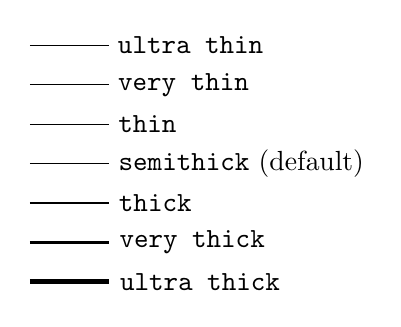
\begin{tikzpicture}
   \draw[ultra thin] (0,0)--(1,0)node[right]{\ttfamily ultra thin};
   \draw[very thin] (0,-.5)--(1,-.5)node[right]{\ttfamily very thin};
   \draw[thin] (0,-1)--(1,-1)node[right]{\ttfamily thin};
   \draw[semithick] (0,-1.5)--(1,-1.5)node[right]{{\ttfamily semithick} (default)};
   \draw[thick] (0,-2)--(1,-2)node[right]{\ttfamily thick};
   \draw[very thick] (0,-2.5)--(1,-2.5)node[right]{\ttfamily very thick};
   \draw[ultra thick] (0,-3)--(1,-3)node[right]{\ttfamily ultra thick};
 \end{tikzpicture}
\end{flushleft}

This command also applies to \cmd{merge}.

\subsection{\cmd{setbondshape}}\label{ssec:setbondshape}
With
\begin{beschreibung}
 \Befehl{setbondshape}{<base length>}\ma{<dash thickness>}\ma{<dash spacing>}
\end{beschreibung}
you can change \cmd{setcrambond}{<base length>}\ma{<dash thickness>}\ma{<dash spacing>}
for all \paket{chemfig} formul\ae\ \emph{inside} of the \mychemistry environments.
Default values are (in this order) \SI{3}{pt}, \SI{.5}{pt} and \SI{1}{pt}. If
you leave an argument empty the value is reset to default.

\subsection{\cmd{setelmove}}\label{ssec:setelmove}
The command
\begin{beschreibung}
 \Befehl{setelmove}{<tikz>}
\end{beschreibung}
sets the default style that is used for the lines drawn by \cmd{elmove}. An empty
argument resets to \code{->,red,shorten <=3pt,shorten >=1pt}.

\subsection{\cmd{setmergelength}}\label{ssec:setmergelength}
With
\begin{beschreibung}
 \Befehl{setmergelength}{<length>}
\end{beschreibung}
you can change the length of the \cmd{merge} arrow. More precisely you can change
the length of the arrow from the point of line crossing to the arrow tip (see
section~\ref{ssec:merge}). If you leave the argument empty the value is reset to
default (\SI{3}{em}).

\subsection{\cmd{setrcndist}}\label{ssec:setrcndist}
The nodes within which the reactants an arrows are set have a certain distance
between them. The default distance is \SI{1}{em}. If you want to change that you
can use
\begin{beschreibung}
 \Befehl{setrcndist}{<length>}
\end{beschreibung}
If you leave the argument empty the distance is reset to \SI{1}{em}.
\begin{beispiel}
 \setrcndist{2em}
 \begin{rxn}
  \reactant{A}\arrow{}{}
 \end{rxn}
 \setrcndist{}
 \begin{rxn}
  \reactant{A}\arrow{}{}
 \end{rxn}
\end{beispiel}

\subsection{\cmd{setrxnalign}/\cmd{setschemealign}}\label{ssec:setrxnalign}\label{ssec:setschemealign}
With the commands
\begin{beschreibung}
 \Befehl{setrxnalign}{<alignment>}
 \Befehl{setschemealign}{<alignment>}
\end{beschreibung}
The default alignment behaviour of \env{rxn}{} and \env{rxnscheme}{} (see
sections~\ref{sssec:rxn_optionen} and \ref{sssec:rxnscheme_optionen}) can be set.
You can choose between \code{left}, \code{center} and \code{right}.

If you leave the argument empty \mychemistry's default behaviour (\code{center})
is restored.
\begin{beispiel}
 \setrxnalign{right}
 \begin{rxn}
  \reactant{A}\arrow{}{}\reactant{B}
 \end{rxn}
 \setrxnalign{}
 \begin{rxn}
  \reactant{A}\arrow{}{}\reactant{B}
 \end{rxn}
\end{beispiel}

\subsection{\cmd{setschemename}}\label{ssec:setschemename}
See page~\pageref{par:rxnscheme_name}.

\subsection{\cmd{transition}}\label{ssec:transition}
\cmd{transition} works exactly like \cmd{reactant} (see section~\ref{ssec:reactant}).
\begin{beschreibung}
 \Befehl{transition}[<pos>,<anchor>,<tikz>]{<formula>}
\end{beschreibung}
\begin{beispiel}
 \begin{rxn}
  \reactant{ \ch{H2 + I2} }
  \arrow[below,<=>,.5]{}{}
  \transition[below]{ \chemfig[dotted][]{H?-I-[2]I-[4]H?} }
  \arrow[below,<=>,.5]{}{}
  \reactant[below]{ \ch{2 HI} }
 \end{rxn}
\end{beispiel}

\appendix
\printindex
\end{document}